\documentclass[10pt,A4paper,tikz,border=10pt]{standalone}
\usepackage[utf8]{inputenc}
\usepackage[T1]{fontenc}
\usepackage{amsmath}
%\usepackage{amsfonts}
\usepackage{amssymb}
\usepackage{mathtools}
\DeclarePairedDelimiter\abs{\lvert}{\rvert}
\usepackage{tikz}
\usetikzlibrary{shapes,arrows,shapes.misc,shapes.symbols}
\usetikzlibrary{positioning}
\usepackage{gitinfo2}
\usepackage{graphicx}

\makeatletter
\AddToShipoutPictureBG{%
	\AtPageLowerLeft{%
		\kern2.6cm
		\raisebox{\dimexpr.5\paperheight-.8\height}
		{\rotatebox{90}{\gitMarkFormat\gitMarkPref{} \textbullet{} \gitMark}}%
	}%
}%
\makeatother
\newcommand{\prdfrazioni}{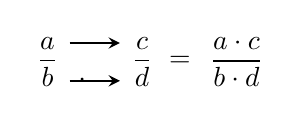
\begin{tikzpicture}[thick]
		\def\x{2.8mm}
		\def\h{2.4mm}
		\def\dist{12mm}%1cm
		\node at (0,0) {$\displaystyle \frac{a}{b}$};
		\node at (\dist,0) {$\displaystyle \frac{c}{d}$};
		\node at (1.4*\dist,0) {$\displaystyle =$};
		\node at (2.0*\dist,0) {$\displaystyle \frac{a\cdot c}{b\cdot d}$};
		% collegamento termini
		\draw[-stealth] (\x, \h)--(\dist-\x,\h); 
		\draw[-stealth] (\x,-\h)--node [near start] {$\cdot$}(\dist-\x, -\h);
	\end{tikzpicture}%
}
%\renewcommand{\gitMarkFormat}{\color{blue}\sffamily\bfseries}
\begin{document}
\tikzset{
	decision/.style={diamond, draw, %fill=blue!20,
		text width=5.5em, text badly centered, 
		%node distance=2.5cm
		, inner sep=0pt
	},
	block/.style={rectangle, draw, %fill=blue!20,
		text width=10em, 
		text centered, 
		%node distance=2.0cm,
		%rounded corners, 
		minimum height=3em
	},
	loop/.style={chamfered rectangle,chamfered rectangle 	xsep=2cm, draw, %fill=blue!20,
		text width=15em, text centered,  
		node distance=2.5cm,% minimum height=3em
	},
	cloud/.style={draw, ellipse,%fill=red!20, 
		%node distance=1.5cm,
		 minimum height=2em
	},
	input/.style={ % requires library shapes.geometric
		draw,
		%node distance=1.5cm,
			text width=10em, text centered,  
		trapezium,
		trapezium left angle=60,
		trapezium right angle=120,
	},
	line/.style={draw, very thick, %color=black!50,
		-latex'},
	print/.style={ % requires library shapes.symbols
		draw,
		text width=10em, 
		text centered,  
		tape,
		tape bend top=none
	},
connessione/.style={
draw,
circle,
radius=5pt,
}
}
%	\begin{center}

		\begin{tikzpicture}[scale=1, %node distance = 2.5cm,
			 auto]
			% Place nodes
			\node [cloud] (init) {Inizio};
			\node[input, below of=init] (pass1) {Leggo il sistema};
			\node[connessione,below of=pass1] (nodo1) {};
			\node[decision,below of=nodo1,node distance=2.5cm ] (dec1) {Il sistema è in forma normale?};
			
		\node [block,  right of=dec1, node distance=4.2cm] (sno1) {Trasformo il sistema in forma normale};
		\node[block, below of=dec1, node distance=3cm] (ssi1) {Scelgo una riga};
		\node[block, below of=ssi1, node distance=2cm] (pass3) {Risolvo la riga rispetto un'incognita};
		\node[block, below of=pass3, node distance=2.5cm] (pass4) {Sostituisco con la soluzione trovata, l'incognita nell'altra riga};
			\node[block, below of=pass4, node distance=2.5cm] (pass5) {Ottengo un'equazione di primo grado in una sola incognita};
		\node[block, below of=pass5, node distance=2cm] (pass6) {Risolvo l'equazione};
	\node[decision, below of=pass6, node distance=3cm] (dec2) {Ho una soluzione?};
	\node[decision, right of=dec2, node distance=3.5cm] (dec3) {Ho un'identità?};
	
	\node [print, right of=dec3,node distance=4cm] (dec3no) {Sistema impossibile};
	\node [print, below of=dec3,node distance=2.5cm] (dec3si) {Sistema indeterminato};
	\node [block, below of=dec2,node distance=4cm] (dec2si) {Sostituisco la soluzione trovata nella riga di partenza};
\node[block, below of=dec2si, node distance=2cm] (pass7) {Ottengo il valore dell'altra incognita};
\node[print,below of=pass7, node distance=2cm] (pass8) {La coppia ottenuta è la soluzione};
\node[connessione,below of=pass8] (nodo2) {};
\node [cloud, below of=nodo2] (stop) {Fine};

			\path [line] (init) -- (pass1);
			\path [line] (pass1) -- (nodo1);
   		\path [line] (nodo1) --  (dec1);
        \path [line] (dec1) -- node[near start] {Si} (ssi1);
         \path [line] (dec1) -- node[near start] {No} (sno1);
         \path [line] (sno1) |-(nodo1);
			\path [line] (ssi1) --  (pass3);
		 \path [line] (pass3) --  (pass4);
		 \path [line] (pass4) --  (pass5);
		 \path [line] (pass5) --  (pass6);
			\path [line] (pass6) --  (dec2);
			\path[line]  (dec2)--node[near start]{No}(dec3);
			\path[line]  (dec3)--node[near start]{No}(dec3no);
			\path[line]  (dec3)--node[near start]{Si}(dec3si);
			\path[line]  (dec2)--node[near start]{Si}(dec2si);
			\path [line] (dec2si) --  (pass7);
			\path [line] (pass7) --  (pass8);
			\path [line] (pass8) --  (nodo2);
			\path [line] (nodo2) --  (stop);
			\path [line] (dec3no) |-  (nodo2);
			\path [line] (dec3si) |-  (nodo2);
%			\path[line] (decisione2.west)--node[near start]{No}++(-3,0)|-(nodo1);
%			\path [line] (decisione2) --node[near start]{Si}  (nodo3);
%			\path [line] (nodo3) --  (passo3);
%			\path[line] (passo3)--(decisione3);
%			\path [line] (decisione3) -- node[near start] {No} (sceltano3);
%			\path [line] (decisione3) -- node[near start] {Si} (sceltasi3);
%			\path[line] (sceltasi3)--(nodo4);
%			\path[line] (sceltano3)|-(nodo4);
%			\path[line] (nodo4)--(decisione4);
%			\path[line] (decisione4.west)--node[near start]{No}++(-3,0)|-(nodo3);
%			\path[line] (decisione4)--(passo4);
%			
%				\path[line] (passo4)--(decisione5);
%				\path[line] (decisione5)--node [near start]{Si}(decisione6);
%				\path[line] (decisione6)--node [near start]{Si}(sceltasi6);
%				\path[line] (decisione6)--node [near start]{No}(sceltano6);
%			\path[line] (decisione5)--node [near start]{No}(sceltano5);
%			\path[line] (sceltano5)--(passo5);
%			\path[line](passo5)|-(nodo5);
%			\path[line] (sceltano6)--(nodo5);
%			\path[line] (sceltasi6)|-(nodo5);
%			\path[line](nodo5)--(stop);
		\end{tikzpicture}
%	\end{center}
\end{document}